% Created by tikzDevice version 0.6.2-92-0ad2792 on 2013-01-08 03:49:56
% !TEX encoding = UTF-8 Unicode
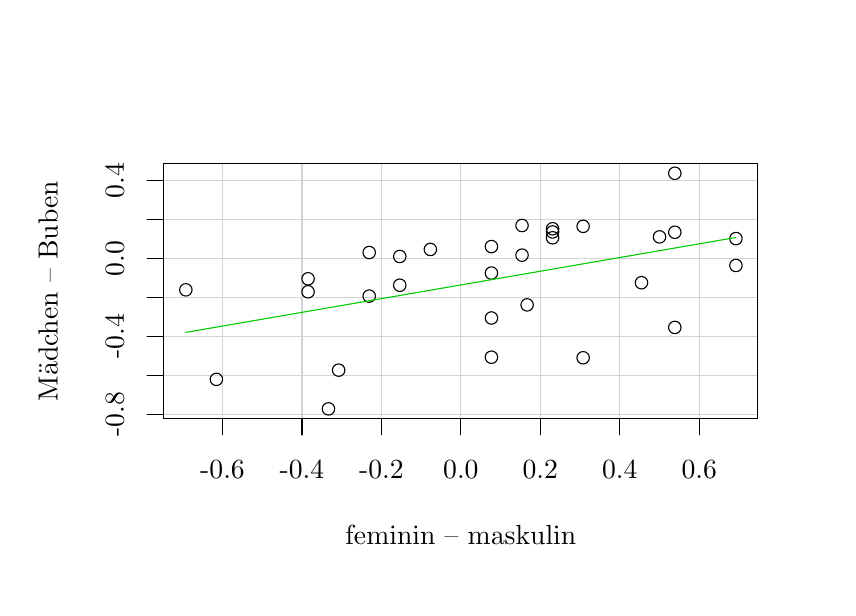
\begin{tikzpicture}[x=1pt,y=1pt]
\definecolor[named]{fillColor}{rgb}{1.00,1.00,1.00}
\path[use as bounding box,fill=fillColor,fill opacity=0.00] (0,0) rectangle (289.08,202.36);
\begin{scope}
\path[clip] (  0.00,  0.00) rectangle (289.08,202.36);
\definecolor[named]{drawColor}{rgb}{0.00,0.00,0.00}

\path[draw=drawColor,line width= 0.4pt,line join=round,line cap=round] ( 70.40, 61.20) -- (242.68, 61.20);

\path[draw=drawColor,line width= 0.4pt,line join=round,line cap=round] ( 70.40, 61.20) -- ( 70.40, 55.20);

\path[draw=drawColor,line width= 0.4pt,line join=round,line cap=round] ( 99.12, 61.20) -- ( 99.12, 55.20);

\path[draw=drawColor,line width= 0.4pt,line join=round,line cap=round] (127.83, 61.20) -- (127.83, 55.20);

\path[draw=drawColor,line width= 0.4pt,line join=round,line cap=round] (156.54, 61.20) -- (156.54, 55.20);

\path[draw=drawColor,line width= 0.4pt,line join=round,line cap=round] (185.25, 61.20) -- (185.25, 55.20);

\path[draw=drawColor,line width= 0.4pt,line join=round,line cap=round] (213.96, 61.20) -- (213.96, 55.20);

\path[draw=drawColor,line width= 0.4pt,line join=round,line cap=round] (242.68, 61.20) -- (242.68, 55.20);

\node[text=drawColor,anchor=base,inner sep=0pt, outer sep=0pt, scale=  1.00] at ( 70.40, 39.60) {-0.6};

\node[text=drawColor,anchor=base,inner sep=0pt, outer sep=0pt, scale=  1.00] at ( 99.12, 39.60) {-0.4};

\node[text=drawColor,anchor=base,inner sep=0pt, outer sep=0pt, scale=  1.00] at (127.83, 39.60) {-0.2};

\node[text=drawColor,anchor=base,inner sep=0pt, outer sep=0pt, scale=  1.00] at (156.54, 39.60) {0.0};

\node[text=drawColor,anchor=base,inner sep=0pt, outer sep=0pt, scale=  1.00] at (185.25, 39.60) {0.2};

\node[text=drawColor,anchor=base,inner sep=0pt, outer sep=0pt, scale=  1.00] at (213.96, 39.60) {0.4};

\node[text=drawColor,anchor=base,inner sep=0pt, outer sep=0pt, scale=  1.00] at (242.68, 39.60) {0.6};

\path[draw=drawColor,line width= 0.4pt,line join=round,line cap=round] ( 49.20, 62.66) -- ( 49.20,147.08);

\path[draw=drawColor,line width= 0.4pt,line join=round,line cap=round] ( 49.20, 62.66) -- ( 43.20, 62.66);

\path[draw=drawColor,line width= 0.4pt,line join=round,line cap=round] ( 49.20, 76.73) -- ( 43.20, 76.73);

\path[draw=drawColor,line width= 0.4pt,line join=round,line cap=round] ( 49.20, 90.80) -- ( 43.20, 90.80);

\path[draw=drawColor,line width= 0.4pt,line join=round,line cap=round] ( 49.20,104.87) -- ( 43.20,104.87);

\path[draw=drawColor,line width= 0.4pt,line join=round,line cap=round] ( 49.20,118.94) -- ( 43.20,118.94);

\path[draw=drawColor,line width= 0.4pt,line join=round,line cap=round] ( 49.20,133.01) -- ( 43.20,133.01);

\path[draw=drawColor,line width= 0.4pt,line join=round,line cap=round] ( 49.20,147.08) -- ( 43.20,147.08);

\node[text=drawColor,rotate= 90.00,anchor=base,inner sep=0pt, outer sep=0pt, scale=  1.00] at ( 34.80, 62.66) {-0.8};

\node[text=drawColor,rotate= 90.00,anchor=base,inner sep=0pt, outer sep=0pt, scale=  1.00] at ( 34.80, 90.80) {-0.4};

\node[text=drawColor,rotate= 90.00,anchor=base,inner sep=0pt, outer sep=0pt, scale=  1.00] at ( 34.80,118.94) {0.0};

\node[text=drawColor,rotate= 90.00,anchor=base,inner sep=0pt, outer sep=0pt, scale=  1.00] at ( 34.80,147.08) {0.4};

\path[draw=drawColor,line width= 0.4pt,line join=round,line cap=round] ( 49.20, 61.20) --
	(263.88, 61.20) --
	(263.88,153.16) --
	( 49.20,153.16) --
	( 49.20, 61.20);
\end{scope}
\begin{scope}
\path[clip] (  0.00,  0.00) rectangle (289.08,202.36);
\definecolor[named]{drawColor}{rgb}{0.00,0.00,0.00}

\node[text=drawColor,anchor=base,inner sep=0pt, outer sep=0pt, scale=  1.00] at (156.54, 15.60) {feminin -- maskulin};

\node[text=drawColor,rotate= 90.00,anchor=base,inner sep=0pt, outer sep=0pt, scale=  1.00] at ( 10.80,107.18) {Mädchen -- Buben};
\end{scope}
\begin{scope}
\path[clip] ( 49.20, 61.20) rectangle (263.88,153.16);
\definecolor[named]{drawColor}{rgb}{0.83,0.83,0.83}

\path[draw=drawColor,line width= 0.4pt,line join=round,line cap=round] ( 70.40, 61.20) -- ( 70.40,153.16);

\path[draw=drawColor,line width= 0.4pt,line join=round,line cap=round] ( 99.12, 61.20) -- ( 99.12,153.16);

\path[draw=drawColor,line width= 0.4pt,line join=round,line cap=round] (127.83, 61.20) -- (127.83,153.16);

\path[draw=drawColor,line width= 0.4pt,line join=round,line cap=round] (156.54, 61.20) -- (156.54,153.16);

\path[draw=drawColor,line width= 0.4pt,line join=round,line cap=round] (185.25, 61.20) -- (185.25,153.16);

\path[draw=drawColor,line width= 0.4pt,line join=round,line cap=round] (213.96, 61.20) -- (213.96,153.16);

\path[draw=drawColor,line width= 0.4pt,line join=round,line cap=round] (242.68, 61.20) -- (242.68,153.16);

\path[draw=drawColor,line width= 0.4pt,line join=round,line cap=round] ( 49.20, 62.66) -- (263.88, 62.66);

\path[draw=drawColor,line width= 0.4pt,line join=round,line cap=round] ( 49.20, 76.73) -- (263.88, 76.73);

\path[draw=drawColor,line width= 0.4pt,line join=round,line cap=round] ( 49.20, 90.80) -- (263.88, 90.80);

\path[draw=drawColor,line width= 0.4pt,line join=round,line cap=round] ( 49.20,104.87) -- (263.88,104.87);

\path[draw=drawColor,line width= 0.4pt,line join=round,line cap=round] ( 49.20,118.94) -- (263.88,118.94);

\path[draw=drawColor,line width= 0.4pt,line join=round,line cap=round] ( 49.20,133.01) -- (263.88,133.01);

\path[draw=drawColor,line width= 0.4pt,line join=round,line cap=round] ( 49.20,147.08) -- (263.88,147.08);
\end{scope}
\begin{scope}
\path[clip] (  0.00,  0.00) rectangle (289.08,202.36);
\definecolor[named]{drawColor}{rgb}{0.00,0.00,0.00}

\path[draw=drawColor,line width= 0.4pt,line join=round,line cap=round] ( 49.20, 61.20) --
	(263.88, 61.20) --
	(263.88,153.16) --
	( 49.20,153.16) --
	( 49.20, 61.20);
\end{scope}
\begin{scope}
\path[clip] ( 49.20, 61.20) rectangle (263.88,153.16);
\definecolor[named]{drawColor}{rgb}{0.00,0.00,0.00}

\path[draw=drawColor,line width= 0.4pt,line join=round,line cap=round] (167.58,123.25) circle (  2.25);

\path[draw=drawColor,line width= 0.4pt,line join=round,line cap=round] (134.45,109.29) circle (  2.25);

\path[draw=drawColor,line width= 0.4pt,line join=round,line cap=round] (134.45,119.68) circle (  2.25);

\path[draw=drawColor,line width= 0.4pt,line join=round,line cap=round] (178.63,120.16) circle (  2.25);

\path[draw=drawColor,line width= 0.4pt,line join=round,line cap=round] (178.63,130.87) circle (  2.25);

\path[draw=drawColor,line width= 0.4pt,line join=round,line cap=round] (200.71,130.57) circle (  2.25);

\path[draw=drawColor,line width= 0.4pt,line join=round,line cap=round] (228.32,126.76) circle (  2.25);

\path[draw=drawColor,line width= 0.4pt,line join=round,line cap=round] (108.69, 64.61) circle (  2.25);

\path[draw=drawColor,line width= 0.4pt,line join=round,line cap=round] (167.58, 83.28) circle (  2.25);

\path[draw=drawColor,line width= 0.4pt,line join=round,line cap=round] ( 68.19, 75.28) circle (  2.25);

\path[draw=drawColor,line width= 0.4pt,line join=round,line cap=round] (167.58, 97.45) circle (  2.25);

\path[draw=drawColor,line width= 0.4pt,line join=round,line cap=round] (112.37, 78.61) circle (  2.25);

\path[draw=drawColor,line width= 0.4pt,line join=round,line cap=round] (200.71, 83.08) circle (  2.25);

\path[draw=drawColor,line width= 0.4pt,line join=round,line cap=round] (233.84, 94.04) circle (  2.25);

\path[draw=drawColor,line width= 0.4pt,line join=round,line cap=round] (180.47,102.19) circle (  2.25);

\path[draw=drawColor,line width= 0.4pt,line join=round,line cap=round] (123.41,105.37) circle (  2.25);

\path[draw=drawColor,line width= 0.4pt,line join=round,line cap=round] (167.58,113.69) circle (  2.25);

\path[draw=drawColor,line width= 0.4pt,line join=round,line cap=round] (145.50,122.22) circle (  2.25);

\path[draw=drawColor,line width= 0.4pt,line join=round,line cap=round] (189.67,126.43) circle (  2.25);

\path[draw=drawColor,line width= 0.4pt,line join=round,line cap=round] (101.32,106.93) circle (  2.25);

\path[draw=drawColor,line width= 0.4pt,line join=round,line cap=round] (255.93,126.15) circle (  2.25);

\path[draw=drawColor,line width= 0.4pt,line join=round,line cap=round] (101.32,111.61) circle (  2.25);

\path[draw=drawColor,line width= 0.4pt,line join=round,line cap=round] (233.84,149.75) circle (  2.25);

\path[draw=drawColor,line width= 0.4pt,line join=round,line cap=round] ( 57.15,107.63) circle (  2.25);

\path[draw=drawColor,line width= 0.4pt,line join=round,line cap=round] (189.67,128.54) circle (  2.25);

\path[draw=drawColor,line width= 0.4pt,line join=round,line cap=round] (233.84,128.43) circle (  2.25);

\path[draw=drawColor,line width= 0.4pt,line join=round,line cap=round] (189.67,129.69) circle (  2.25);

\path[draw=drawColor,line width= 0.4pt,line join=round,line cap=round] (255.93,116.43) circle (  2.25);

\path[draw=drawColor,line width= 0.4pt,line join=round,line cap=round] (221.80,110.19) circle (  2.25);

\path[draw=drawColor,line width= 0.4pt,line join=round,line cap=round] (123.41,121.11) circle (  2.25);
\definecolor[named]{drawColor}{rgb}{0.00,0.80,0.00}

\path[draw=drawColor,line width= 0.4pt,line join=round,line cap=round] ( 57.15, 92.25) --
	(255.93,126.54);
\end{scope}
\end{tikzpicture}
